 \section{Translator}\label{sec:translator}

 We develop a dedicated translator to convert \conesc code to plain
 nesC. To do so, our translator performs two passes through the input
 code. First, it reads the main \code{Makefile} to determine the main
 configuration component and to recursively scan the component
 tree. Based on the information gained during the first pass,
 including the list of every context and context groups defined in the
 code, it parses every input file to convert the \conesc code to plain
 nesC and to generate a set of support functionality. The resulting
 sources are then compiled using the standard nesC toolchain to
 produce a deployment-ready binary.

\putfigure{caption=\conesc translation to nesC code for a generic \code{FooGroup} context group and an individual context \code{FooCon}.,label=fig:ctd}{
 \centering
 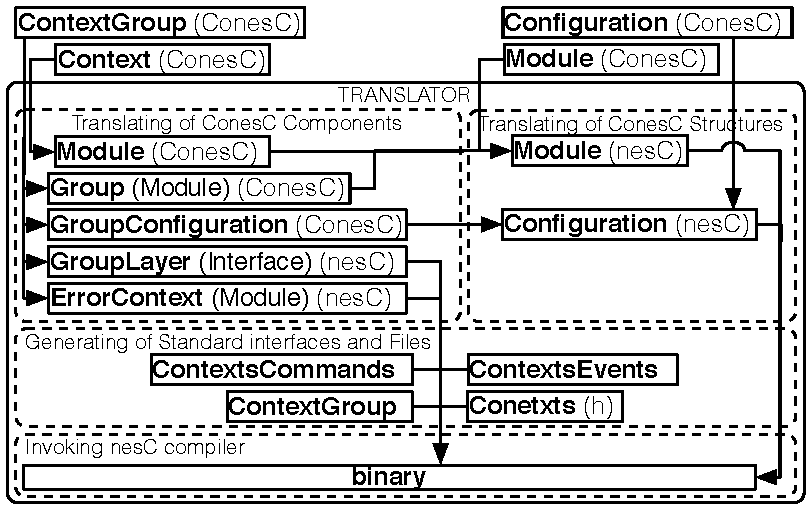
\includegraphics[width=\columnwidth]{pdf/translator}
}

Fig.~\ref{fig:ctd} details the operations during the second
pass. Generally, the input to the translator includes four types of
components: context groups and contexts, as well as nesC
configurations and modules where \conesc constructs appear.  In
Fig.~\ref{fig:ctd}, context groups and contexts are represented by a
sample \code{FooGroup} context group and an individual \code{FooCon}
context, whereas nesC configurations (modules) with \conesc
constructs are represented as \code{BarC} (\code{BarP}).

Based on every context group, we generate a custom nesC module, such
as \code{FooGroupBinding} in Fig.~\ref{fig:ctd}, that implements the
dynamic binding of layered functions to the active context. This
module is part of a configuration, such as \code{FooGroupConfig} in
Fig.~\ref{fig:ctd}, also automatically generated. This configuration
implements a nesC interface our translator produces, such as
\code{FooGroupLayered} in Fig.~\ref{fig:ctd}, that exports the layered
functions defined in the group. Optionally, an error context is also
generated in plain nesC, as indicated by \code{ErrorFooGroup} in this
case, if the programmer does not provide one. Each individual context
is translated to a corresponding nesC module with the proper
interfaces to be wired within the aforementioned configuration, as in
the case of \code{FooConContext} for the \code{FooGroupConfig} in
Fig.~\ref{fig:ctd}.

At this stage, context and context groups disappeared, yet \conesc
constructs, such as \code{activate}, may still appear within the
source code. Our translator converts these constructs to
functionally-equivalent nesC code both in the nesC files generated out
of context groups and individual contexts, and in the plain nesC files
that possibly includes them, such as \code{BarC} and \code{BarP} in
Fig.~\ref{fig:ctd}. The resulting sources are then wired to generic
interfaces that define the predefined commands and events in \conesc,
such as \code{contextChanged} for context groups, as in
Fig.~\ref{fig:mm}, and \code{activated/deactivated} for individual
contexts, as in Fig.~\ref{fig:irc} and~\ref{fig:cc}. The result is
plain nesC code that can be given as input to the nesC toolchain.

% \putfigure{caption=Hierarchy of generated components.,label=fig:gfh}{
%  \centering
%  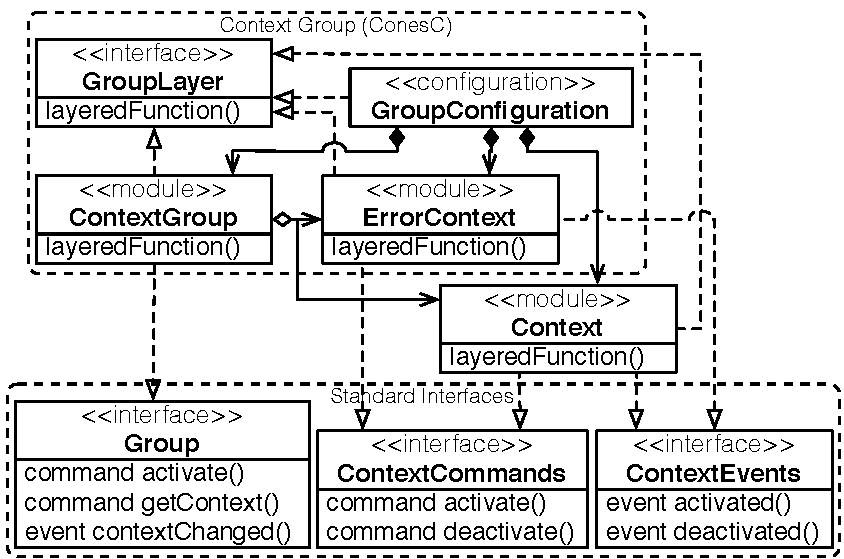
\includegraphics[width=\columnwidth]{pdf/architecture}
% }

% The hierarchy of generated based on \emph{context group} components is displayed
% in Fig.~\ref{fig:gfh}. \emph{GroupLayer} -- a basic interface for all generated
% components -- declares a \emph{layered function}. \emph{GroupConfiguration} is a
% main component, which instantiates \emph{ConetxtGroup} and declared
% \emph{contexts}, and glue them together. The former implements all the internal
% logic to operate by \emph{contexts} and enable behavioral variation.
% \emph{ErrorContext} module is generated if it was not declared in the
% \emph{context group}. \emph{Context} is translated into module by adding
% standard functions and implementation of \emph{group layer} interface mentioned
% above.

% The generated components and written by a developer modules are translated then
% from \conesc into nesC. After that the translator generates standard interfaces
% for additional functionality -- e.g. activation and deactivation of contexts --
% for \emph{ContextGroup} and \emph{contexts}. \emph{Contexts.h} is a definition
% of all the contexts in the projects. The last step is invoking the nesC compiler
% to build a binary by using all the generated and transformed components.

Our translator is implemented using JavaCC~\cite{javacc}. Two aspects
are worth noticing. First, the generated code is completely
hardware-independent. Therefore, hardware compatibility is the same as
the original nesC toolchain, allowing us to support a wide range of
WSN platforms and not to modify our translator due to hardware
idiosyncrasies. Second, the whole translation process is only
seemingly straightforward. Rendering the logic embedded within the
\conesc abstractions does require a fairly sophisticated
processing. To give an intuition, we measured the size of the \conesc
implementations of the application we use for evaluation, described
next, against the size of the nesC implementations output by our
translator. On average, we observe three times as much lines of code
in the automatically-generated nesC code.

%%% Local Variables: 
%%% mode: latex
%%% TeX-master: "bare_conf"
%%% End: 
